\documentclass[a4paper,english,12pt]{article}
\usepackage{%
	amsfonts,%
	amsmath,%	
	amssymb,%
	amsthm,%
	algorithm,%
	babel,%
	bbm,%
	etex,%
	%biblatex,%
	caption,%
	centernot,%
	color,%
	dsfont,%
	enumerate,%
	epsfig,%
	epstopdf,%
	geometry,%
	graphicx,%
	hyperref,%
	latexsym,%
	mathtools,%
	multicol,%
	pgf,%
	pgfplots,%
	pgfplotstable,%
	pgfpages,%
	proof,%
	psfrag,%
	subfigure,%	
	tikz,%
	ulem,%
	url%
}	
\usepackage[noend]{algpseudocode}
\usepackage[mathscr]{eucal}
\usepgflibrary{shapes}
\usetikzlibrary{%
  	arrows,%
	backgrounds,%
	chains,%
	decorations.pathmorphing,% /pgf/decoration/random steps | erste Graphik
	decorations.text,%
	matrix,%
  	positioning,% wg. " of "
  	fit,%
	patterns,%
  	petri,%
	plotmarks,%
  	scopes,%
	shadows,%
  	shapes.misc,% wg. rounded rectangle
  	shapes.arrows,%
	shapes.callouts,%
  	shapes%
}

\theoremstyle{plain}
\newtheorem{thm}{Theorem}[section]
\newtheorem{lem}[thm]{Lemma}
\newtheorem{prop}[thm]{Proposition}
\newtheorem{cor}[thm]{Corollary}

\theoremstyle{definition}
\newtheorem{defn}[thm]{Definition}
\newtheorem{conj}[thm]{Conjecture}
\newtheorem{exmp}[thm]{Example}
\newtheorem{assum}[thm]{Assumptions}
\newtheorem{axiom}[thm]{Axiom}

\theoremstyle{remark}
\newtheorem{rem}{Remark}
\newtheorem{note}{Note}
\newtheorem{fact}{Fact}

\newcommand{\norm}[1]{\left\lVert#1\right\rVert}
\newcommand{\indep}{\!\perp\!\!\!\perp}
\DeclarePairedDelimiter\abs{\lvert}{\rvert}%
\newcommand\numberthis{\addtocounter{equation}{1}\tag{\theequation}}
\newcommand{\tr}{\operatorname{tr}}
\newcommand{\R}{\mathbb{R}}
\newcommand{\N}{\mathbb{N}}
\newcommand{\E}{\mathbb{E}}
\newcommand{\Z}{\mathbb{Z}}
\newcommand{\B}{\mathscr{B}}
\newcommand{\C}{\mathcal{C}}
\newcommand{\T}{\mathscr{T}}
\newcommand{\F}{\mathcal{F}}
\newcommand{\G}{\mathcal{G}}
%\newcommand{\ba}{\begin{align*}}
%\newcommand{\ea}{\end{align*}}
\DeclareMathOperator*{\argmax}{arg\,max}
\renewcommand{\qedsymbol}{$\blacksquare$}
\makeatletter
\def\BState{\State\hskip-\ALG@thistlm}
\makeatother

\makeatletter
\def\th@plain{%
  \thm@notefont{}% same as heading font
  \itshape % body font
}
\def\th@definition{%
  \thm@notefont{}% same as heading font
  \normalfont % body font
}
\makeatother
\date{}
%\usepackage{amsfonts}
%\usepackage{graphicx}
%\usepackage[top=1.2in,bottom=1.2in,left=1in,right=1in]{geometry}
\title{Lecture-5: Composite Hypothesis Testing}
\date{22 Jan 16}
\begin{document}
\maketitle
\begin{exmp}{Neyman-Pearson Hypothesis Testing for binary channel (contd. from previous lecture)}
\par Decision rule for Neyman Pearson testing has the form,
\begin{equation}
\tilde{\delta}_{NP} (y)=
\begin{cases}
1,\hspace{10pt}L(y) > \eta_0,\\ 
\gamma_0,\hspace{5pt}L(y)= \eta_0,\\
0,\hspace{10pt}L(y) < \eta_0,\\
\end{cases}
\end{equation}
where $\eta_0$ is desired threshold for $\alpha$ level Neyman Pearson testing, and $ L(y) = \frac{{P}_1(y)}{{P}_0(y)} $ is the likelihood ratio. For the case of binary communication channel example (fig. \ref{fig:BSC}), we have,
\begin{figure}
\centering
\begin{tikzpicture}[scale=4]				
\draw (-0.05,0) node {${\bf 1}$} (0,0) -- (1,0) (1.05,0) node {${\bf 1}$}
node [below,midway,sloped] (TextNode) {$1-\lambda_1$};
\draw (-0.05,0.5) node {${\bf 0}$} (0,0.5) -- (1,0.5) (1.05,0.5) node {${\bf 0}$} node [above,midway,sloped] (TextNode) {$1-\lambda_0$};    
\draw (0,0) -- (1,0.5) node [pos=0.8,below] (TextNode) {$\lambda_1$} ;    
\draw (0,0.5) -- (1,0) node [pos=0.8,above] (TextNode) {$\lambda_0$} ;    
\end{tikzpicture}
\caption{The Binary Channel}
\label{fig:BSC}
\end{figure}
\begin{equation}
%L(0) = \frac{\mathbb{P}_1(0)}{\mathbb{P}_0(0)} = \frac{\lambda_1}{1-\lambda_0} ; \\
%L(1) = \frac{\mathbb{P}_1(1)}{\mathbb{P}_0(1)} = \frac{1-\lambda_1}{\lambda_0};\\
L(y) = \begin{cases}
\frac{\lambda_1}{1-\lambda_0},\hspace{5pt}y=0,  \\ 
\frac{1-\lambda_1}{\lambda_0},\hspace{5pt}y=1.
\end{cases}
\end{equation}
Assuming $\lambda_0 + \lambda_1 < 1$, we have,
$\frac{\lambda_1}{1-\lambda_0} < 1$, and $ \frac{1-\lambda_1}{\lambda_0} > 1$. 
\par Now, we get,
\begin{equation}
{P}_0 (L(y) > \eta)=\begin{cases}
1\hspace{10pt}\mbox{if}\hspace{3pt}\eta< \frac{\lambda_1}{1-\lambda_0},\\ 
\lambda_0\hspace{5pt}\mbox{if}\hspace{3pt}\frac{\lambda_1}{1-\lambda_0} \leq \eta \geq \frac{1-\lambda_1}{\lambda_0},\\
0\hspace{10pt}\mbox{if}\hspace{3pt}\eta \geq  \frac{1-\lambda_1}{\lambda_0}.
\end{cases}
\end{equation}
\begin{figure}[t]
\centering
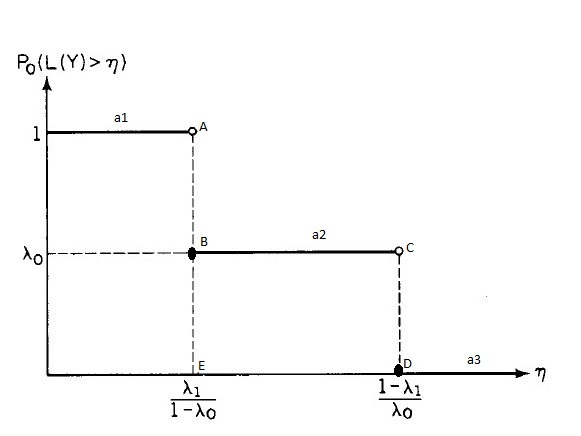
\includegraphics[scale=0.8]{Figures/img.jpg} 
\caption{Curve for threshold and randomization selection for a binary channel.}
\label{fig:pfa}
\end{figure}
Figure \ref{fig:pfa} shows a plot of the probability of false alarm. Let $\eta_0$ be the smallest number such that,
\begin{equation}
{P}_0(p_1(Y) > \eta_0 p_0(Y)) \leq \alpha.
\end{equation}
\begin{equation}
\eta_0 =\begin{cases}
\frac{1-\lambda_1}{\lambda_0},\hspace{10pt}\alpha \in [0,\lambda_0),~~\mbox{(section $a_3$)}\\
\frac{\lambda_1}{1-\lambda_0},\hspace{10pt}\alpha \in [\lambda_0,1),~~\mbox{(section $a_2$)}\\
\mbox{arbitrary},\hspace{10pt}\alpha = 1.
\end{cases}
\end{equation}
If ${P}_0(p_1(Y) > \eta_0 p_0(Y)) <\alpha$, choose  
\begin{equation}
\gamma_0 = \frac{\alpha-{P}_0(p_1(Y) > \eta_0 p_0(Y))}{{P}_0(p_1(Y) = \eta_0 p_0(Y))}
\end{equation}
If $\alpha \in [0,\lambda_0)$,
\begin{equation}
\gamma_0 = \frac{\alpha-0}{{P}_0(p_1(Y) = \eta_0 p_0(Y))}
\end{equation}
and,
\begin{equation}
{P}_0(p_1(Y) = \eta_0 p_0(Y)) = \lambda_0-0
\end{equation}
which is equal to the size of the discontinuity at threshold (CD in fig. \ref{fig:pfa}).
\begin{equation}
\gamma_0 = \frac{\alpha}{\lambda_0}
\end{equation}
If $\alpha \in [\lambda_0,1)$,
\begin{equation}
{P}_0(p_1(Y) = \eta_0 p_0(Y)) = 1-\lambda_0
\end{equation}
which is the size of the discontinuity at threshold (AB in fig. \ref{fig:pfa}). We get, $\gamma_0 = \frac{\alpha-\lambda_0}{1-\lambda_0}$.
\begin{equation}
\gamma_0=\begin{cases}
\frac{\alpha}{\lambda_0},\hspace{45pt}\alpha \in [0,\lambda_0),\\
\frac{\alpha-\lambda_0}{1-\lambda_0},\hspace{32pt}\alpha \in [\lambda_0,1),\\
\mbox{arbitrary},\hspace{10pt}\alpha = 1.
\end{cases}
\end{equation}
If $\alpha \in [0,\lambda_0)$, 
\begin{equation}
\tilde{\delta}_{NP} (y) =\begin{cases}
\frac{\alpha}{\lambda_0},\hspace{10pt}\mbox{if}~y=1,\\
0,\hspace{15pt}\mbox{if}~y=0.\\
\end{cases}
\end{equation}
If $\alpha \in [\lambda_0,1]$,
\begin{equation}
\tilde{\delta}_{NP} (y) =\begin{cases}
1,\hspace{32pt}\mbox{if}~y=1,\\
\frac{\alpha - \lambda_0}{1-\lambda_0},\hspace{15pt}\mbox{if}~y=0.\\
\end{cases}
\end{equation}
The detection probability of the Neyman-Pearson test is given by ,
\begin{eqnarray}
{P}_D (\tilde{\delta}_{NP}) ={P}_1(L(Y) > \eta_0) + \gamma_0 {P}_1(L(Y) = \eta_0),\\\nonumber
{P}_D (\tilde{\delta}_{NP}) =\begin{cases}
\frac{\alpha (1-\lambda_1)}{\lambda_0},\hspace{80pt}\alpha \in [0,\lambda_0),\\
(1-\lambda_1) + \frac{\lambda_1 (\alpha -\lambda_0)}{1-\lambda_0},\hspace{20pt}\alpha \in [\lambda_0,1].
\end{cases}
\end{eqnarray}
\end{exmp}
\section{Composite Hypothesis Test}
Hypothesis testing problems discussed in the previous lectures are sometimes known as 'simple hypothesis testing problems', because, each of the two hypotheses correspond to only a single distribution for the observation. In many hypothesis testing problems, however, there are many possible distributions that can occur under each of the hypotheses. Hypotheses of this type are known as \textit{Composite Hypotheses}.
\par To model the most general type of composite hypothesis testing problems, we consider a family of probability distributions on $\Gamma$ indexed by a parameter $\theta$ taking values in a parameter set $\Lambda$ (the set of all possible natures of state), $\{P_\theta;~\theta \in \Lambda\}$.
\begin{exmp}
For the simple hypothesis test $\Lambda$ =\{0,1\}. More generally,we might have a parameter space that is the union of two disjoint parameter sets $\Lambda_0$ and $\Lambda_1$ representing the ranges of the parameter under the two hypotheses. 
\end{exmp}
\subsection*{Bayesian Formulation:}
In Bayesian formulation of the composite hypothesis testing problem, the parameter is assumed to be a random quantity, $\Theta$, taking on the values in the set $\Lambda$, $\Theta \in \Lambda$. The distribution $P_\theta$ is interpreted as the conditional distribution of Y given that $\Theta = \theta$.
\begin{equation}
P_\theta \{ Y = y \} = P\{ Y=y | \Theta = \theta\} 
\end{equation}
we will consider only non-randomized decision rules, i.e., $\theta \in \Lambda_0~~\mbox{or}~~\Lambda_1$. To choose an optimum decision rule, assign cost to our decisions through a cost function $ C_i (\theta)$, where, $ C_i (\theta)$ is the cost of choosing decision $i \in \{0,1\}$ when $Y \sim P_\theta$. Assume that $C$ is nonnegative and bounded. 
\par For a decision rule $\delta$, the conditional risk is defined as,
\begin{eqnarray}
R_\theta (\delta) = \mathbb{E}_\theta [ C_{ \delta(Y) } (\theta)],
\end{eqnarray}
where $\mathbb{E}_\theta$ denotes expectation assuming that $ Y \sim P_\theta$. Average Bayes risk is defined as 
\begin{equation}
r(\delta) = \mathbb{E} [ R_\Theta (\delta)].
\end{equation}
Bayes rule defined as minimization of $r(\delta)$.
\begin{align}
r(\delta) &= \mathbb{E} [ R_\Theta (\delta)],\\\nonumber
&= \mathbb{E}[\mathbb{E}_\theta[ C_{ \delta(Y) } (\Theta)| \Theta=\theta ]],\\\nonumber
&= \mathbb{E}[\mathbb{E}[ C_{ \delta(Y) } (\Theta)| \Theta ]],\\\nonumber
&= \mathbb{E}[ C_{ \delta(Y) } (\Theta) ],\\\nonumber
&= \mathbb{E}[\mathbb{E}[ C_{ \delta(Y) } (\Theta) | Y=y ]]\hspace{10pt} \forall \{ y \in \Gamma \},
\end{align}
where the last step uses the relation of iterated expectations, $\mathbb{E}\{X\}=\mathbb{E}\{\mathbb{E}\{X|Y\}\}$. Minimizing $r(\delta)$ is same as minimizing $\mathbb{E}[\mathbb{E}[ C_{ \delta(Y) } (\Theta) | Y=y ]$. Since $\delta(y) $ can only be $0$ or $1$, we see that Bayes rule is given by, 
\begin{equation}
\delta(y) = \underset{i \in \{0,1\}}{\arg\min}~\mathbb{E}[C_i (\Theta) | Y=y].
\end{equation}
We choose $\delta (y)$ to be the decision that minimizes the posterior cost.
\begin{equation}
\delta(y) =\mathbbm{1}_{\{\mathbb{E}[C_1(\Theta) | Y=y] < \mathbb{E}[C_0(\Theta) | Y=y]\}},
\end{equation} 
i.e., $\delta (y)$ chooses the hypothesis that is least costly, on the average, given the observations. For example, when $\Lambda =\{0,1\}$, $\delta (y)$ reduces to the Bayes rule for simple hypothesis test. Assume costs being uniform over the sets $\Lambda_0$, $\Lambda_1$, i.e., $C_i (\theta) = C_{ij},~\forall\theta \in \Lambda_j$, we have,
\begin{multline}
C_{11} {P}(\Theta \in \Lambda_1  | Y=y)  + C_{10}  {P}(\Theta \in \Lambda_0  | Y=y),\\\nonumber
< C_{01} {P}(\Theta \in \Lambda_1  | Y=y)+C_{00}  {P}(\Theta \in \Lambda_0  | Y=y).
\end{multline}
Assuming $ C_{11} < C_{01}$, we get,
\begin{equation}
\Gamma_1 =\left\{y\in \Gamma \left| \frac{C_{10}-C_{00}}{C_{01}-C_{11}} < \frac{\mathbb{P}(\Theta \in \Lambda_1  | Y=y)}{\mathbb{P}(\Theta \in \Lambda_0  | Y=y)} \right.\right\}
\end{equation}
where ${P}(\Theta \in \Lambda_j  | Y=y)$ denotes the conditional probability that $\Theta$ lies in $\Lambda_j$ given that $Y=y$. Assume $Y$ has conditional densities $p(y | \Theta \in \Lambda_j)$ for $j\in\{0,1\}$. Using Bayes rule, we get, 
\begin{equation}
P( \Theta \in \Lambda_j | Y=y) = \frac{{p(Y=y | \Theta \in \Lambda_j)}{P(\Theta \in \Lambda_j)}}{p(y)},~j\in\{0,1\}.
\end{equation}
We can write $\Gamma_1$ as, 
\begin{equation}
\Gamma_1 =\left\{y\in \Gamma \left|  \frac{{p(Y=y | \Theta \in \Lambda_1)}{P(\Theta \in \Lambda_1)}}{{p(Y=y | \Theta \in \Lambda_0)}{P(\Theta \in \Lambda_0)}} > \frac{C_{10}-C_{00}}{C_{01}-C_{11}}\right. \right\}.
\end{equation}
For general case, let $\Theta \sim W,~Y\sim \mathbb{P}_\theta,~\theta \in \Lambda $,
\begin{equation}
d{P}[Y\leq y | \Theta \in \Lambda_j] = \int\limits_{-\infty}^{y}\int_\Lambda {{P}_\theta(y) dW_j(\theta)},
\end{equation}
where,
\begin{equation}
dW_j(\theta)\begin{cases}
0,\hspace{50pt}\theta \notin \Lambda_j,\\
\frac{dW(\theta)}{\mathbb{P}\{\theta \in \Lambda_j\}},\hspace{20pt}\theta \in \Lambda_j.
\end{cases}
\end{equation}
\end{document}